\documentclass[__minimum__.tex]{subfiles}

\begin{document}

\begin{comment}
+ 1) Закон Киргофа
+ 2) Закон смещения Вина
+ 3) Закон Стефана Больцмана
+ 4) Формула Рэлея-Джинса
+ 5) Формула Планка
+ 6) Соотношение неопределенностей Гейзенберга
+ 7) Постулаты квантовой механики
+ 8) Коммутатор
+ 9) Эрмитов оператор
+ 10) Постулат о вещественных велечинах
+ 11) Постулат об измерениях
+ 12) Наблюдаемый оператор
+ 13) Равенство Парсевалля
+ 14) Квантомеханические средние
+ 15) Временное и стационарное уравнения Шредингера
+ 16) Вектор плотности тока вероятности
+ 17) Теорема Эренфеста
+ 18) Дуальное пространство
+ 19) Коммутационные соотношения
+ 20) Кванто-механический гармонический осцилятор
+ 21) Постулаты Бора
+ 22) Полный и собственный момент импульса
23) Матрицы Паули
\end{comment}

\ssection{C Электростатика}

Электрический диполь: электрический дипольный момент, потенциальная энергия диполя в электростатическом поле, момент сил, действующих на диполь в однородном электростатическом поле.\\

\textbf{Электрический диполь} — идеализированная электронейтральная система, состоящая из точечных и равных по абсолютной величине положительного и отрицательного электрических зарядов.

Другими словами, электрический диполь представляет собой совокупность двух равных по абсолютной величине разноимённых точечных зарядов, находящихся на некотором расстоянии друг от друга

Произведение вектора $ \vec l$, проведённого от отрицательного заряда к положительному, на абсолютную величину зарядов $ q\,,$ называется \textbf{дипольным моментом}: $\vec d=q\vec l$.

Во внешнем электрическом поле $\vec E$ на электрический диполь действует момент сил ${\vec d}\times{\vec E}$, который стремится повернуть его так, чтобы дипольный момент развернулся вдоль направления поля.

Потенциальная энергия электрического диполя в (постоянном) электрическом поле равна $-{\vec E}\cdot{\vec d}$. (В случае неоднородного поля это означает зависимость не только от момента диполя - его величины и направления, но и от места, точки нахождения диполя).

Вдали от электрического диполя напряжённость его электрического поля убывает с расстоянием $R$ как $R^{-3}$, то есть быстрее, чем у точечного заряда ( $E \sim R^{-2}$).

Любая в целом электронейтральная система, содержащая электрические заряды, в некотором приближении (то есть собственно в дипольном приближении) может рассматриваться как электрический диполь с моментом $\vec d = \sum_i q_i {\vec r}_i$, где $q_{i}$ — заряд $i$-го элемента, ${\vec r}_i$ — его радиус-вектор. При этом дипольное приближение будет корректным, если расстояние, на котором изучается электрическое поле системы, велико по сравнению с её характерными размерами.
\\
Найдём \textbf{потенциальную энергию}, которой обладает диполь во внешнем электрическом поле (см. Рисунок 1). Эта энергия будет равна:

\begin{equation}
    \textit{П} = q\varphi_+ - q\varphi_- = q(\varphi_+ - \varphi_-),
    \llabel{eq:1}
\end{equation}

где $\varphi_+$ и $\varphi_-$ - значения потенциалов внегнего поля в точках, где находятся заряды $+q$ и $-q$.

\begin{equation}
    \varphi_+ - \varphi_- = \frac{d\varphi}{dx} \Delta x = \frac{d\varphi}{dx} l \cos \alpha.
    \llabel{eq:2}
\end{equation}

\begin{figure}[h]
    \centering
    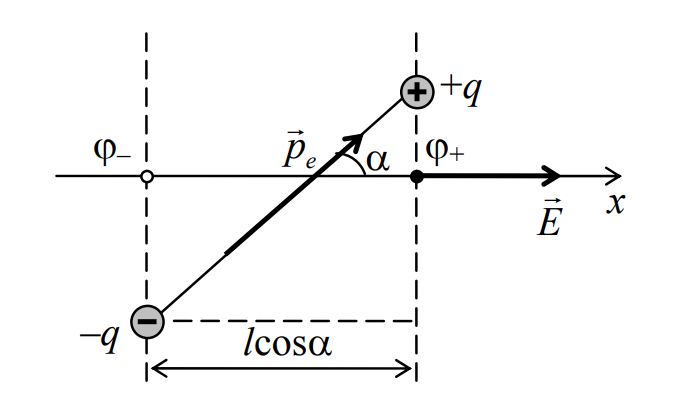
\includegraphics[width=.4\linewidth]{img/e01_1.png}
    \caption{ }
    \llabel{fig:1}
\end{figure}

Подставив выражение (\lref{eq:2}) в (\lref{eq:1}) и учитывая, что $E = -\frac{d\varphi}{dx}$, получим:

\begin{equation}
    \textit{П} = q\frac{d\varphi}{dx} l \cos \alpha = -qEl\cos \alpha = -p_e E \cos \alpha
    \llabel{eq:3}
\end{equation}

Так как угол $\alpha$ в формуле (\lref{eq:3}) - это угол между векторами $\vec{E}$ и $\vec{p_e}$, то данное выражение можно записать в виде:

\begin{equation}
    \textit{П} = - \vec{p_e} \vec{E}
    \llabel{eq:4}
\end{equation}

Выражение (\lref{eq:4}) не учитывает энергию взаимодействия зарядов $+q$ и $-q$, образующих диполь.

Рассмотрим поведение диполя во внешнем электрическом поле. Если диполь поместить в однородное электрическое поле, образующие диполь заряды $+q$ и $-q$ окажутся под дейстивем равных по величине, но противоположных по направлению сил $\vec{F_1}$ и $\vec{F_2}$ (см. Рис. \lref{fig:2}).
\textbf{Момент пары сил}, действующих на диполь, будет равен:

\begin{equation}
    M = Fd = Fl\sin \alpha = qEl\sin \alpha = p_e E \sin \alpha,
    \llabel{eq:5}
\end{equation}
где $d = l\sin \alpha$ - момент пары сил.

\begin{figure}[h]
    \centering
    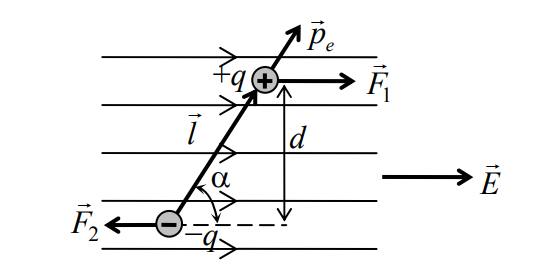
\includegraphics[width=.4\linewidth]{img/e01_2.png}
    \caption{ }
    \llabel{fig:2}
\end{figure}

Формулу (\lref{eq:5}) можно записать в векторном виде:

\begin{equation}
    \vec{M} = \vec{p_e} \times \vec{E}.
\end{equation}

Момент сил стремится повернуть диполь так, чтобы его электрический момент $\vec{p_e}$ установился по направлению поля.

\textbf{Закон Кулона:} Для постоянного электрического поля уравнения Максвелла имеют вид:
$$
\begin{cases}
\operatorname{div}\vec{E} = 4 \pi \rho\\
\operatorname{rot}\vec{E} = 0\\
\end{cases}
$$
Абсолютная величина напряженности поля $E$ будет зависеть только от расстояния $R$ до заряда $e$. Для нахождения этой абсолютной величины применим уравнение
$$
    \operatorname{div}\vec{E}=4\pi\rho
$$
в интегральной форме
$$
    \oint\vec{E}df=4\pi\int\rho dV.
$$
Поток электрического поля через шаровую поверхность с радиусом $R$, проведенную вокруг заряда $e$, равен $4\pi R^2 E$; этот поток должен быть равен $4\pi e$. Тогда:
$$
    E=\frac{e}{R^2}
$$
В векторном виде:
$$
    \vec{E}=\frac{e \vec{R}}{R^3}
$$
Это и есть \textbf{закон Кулона} (Поле, создаваемое точечным зарядом, обратно пропорционально квадрату расстояния до этого заряда)
Напряженность поля. Силу первого рода, отнесенную к заряду, равному единице, называют \textbf{напряженностью электрического поля}:\\
$$
    \vec{E} = -\frac{1}{c}\frac{\partial \vec{A}}{\partial t}-\nabla\varphi,
$$
где $\vec{A}$ -- векторный потенциал поля. Для того чтобы описать электрическое поле, нужно задать вектор напряженности в каждой точке поля. Это можно сделать аналитически или графически. Для этого пользуются \textbf{силовыми линиями} -- это линии, касательная к которым в любой точке поля совпадает с направлением вектора напряженности $\vec{E}$:
\begin{figure}[h]
\centering
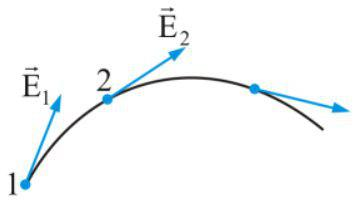
\includegraphics[width=.4\linewidth]{img/С-03_1.jpg}
\end{figure}
Для системы зарядов, как видим, силовые линии направлены от положительного заряда к отрицательному:
\begin{figure}[h]
\centering
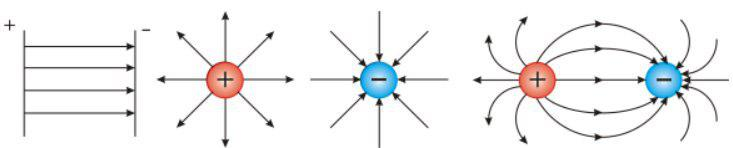
\includegraphics[width=.4\linewidth]{img/С-03_2.jpg}
\end{figure}
\textbf{Эквипотенциальные поверхности} -- это воображаемые поверхности все точки которой имеют одинаковый потенциал.
\begin{gather*}
    U(x,y,z) = const
\end{gather*}
\textbf{Электростатическая защита} -- защита приборов и оборудования, основанная на том, что напряженность электростатического поля внутри проводника равна нулю.\\
Потенциал электростатического поля:
$$
    \varphi=\frac{e}{R}
$$
Работа поля по перемещению заряда из одной точки в другую, называется разностью потенциалов.\\

\emph{Энергия системы точечных зарядов:} рассмотрим систему двух точечных зарядов $q_1$ и $q_2$. Когда заряды бесконечно удалены друг от друга они не взаимодействуют, следовательно, положим их потенциальную энергию равной нулю. Сблизим их на расстояние $r_{12}$, при этом совершится работа для переноса $q_1$:
\begin{gather}
A_{1}=q_{1}\varphi_{1}=q_{1}\frac{1}{4\pi\varepsilon_{0}}\frac{q_2}{r_{12}},
\end{gather}
где $\varphi_{1}$ -- потенциал, создаваемый $q_{2}$ в точке, в которую перемещается $q_{1}$. Аналогично для $q_{2}$:
\begin{gather}
A_{2}=q_{2}\varphi_{2}=q_{2}\frac{1}{4\pi\varepsilon_{0}}\frac{q_{1}}{r_{12}},
\end{gather}
значения $A_{1}$ и $A_{2}$ одинаковы и выражает энергию системы $W$:
\begin{gather}
W=q_{1}\varphi_{1}=q_{2}\varphi_{2}
=
\frac{1}{2}\left(q_{1}\varphi_{1}+q_{2}\varphi_{2}\right),
\llabel{s14:two}
\end{gather}
формула (\lref{s14:two}) выражает \emph{энергию системы двух зарядов}.

Перенесем из бесконечности заряд $q_{3}$ и расположим их на расстоянии $r_{13}$ и $r_{23}$ от $q_{1}$ и $q_{2}$ соответственно, при этом совершим работу:
\begin{gather}
A_{3}=q_{3}\varphi_{3}=q_{3}\frac{1}{4\pi\varepsilon_{0}}\left(\frac{q_1}{r_{13}}+\frac{q_{2}}{r_{23}}\right),
\end{gather}
где $\varphi_{3}$ -- потенциал, создаваемый зарядами $q_1$ и $q_2$ в точке, в которую помещен $q_3$. Сумма работ $A_1$, $A_2$ и $A_3$ равна энергии системы:
\begin{flalign}
\begin{split}
W
=&
\frac{1}{4\pi\varepsilon_{0}}\frac{q_1q_2}{r_{12}}
+
q_{3}\frac{1}{4\pi\varepsilon_{0}}\left(\frac{q_1}{r_{13}}+\frac{q_{2}}{r_{23}}\right)
=\\
=&
\frac{1}{2}\frac{1}{4\pi\varepsilon_{0}}
\left[
q_1\left(\frac{q_2}{r_{12}}+\frac{q_3}{r_{13}}\right)
+
q_2\left(\frac{q_1}{r_{12}}+\frac{q_3}{r_{23}}\right)
+
q_3\left(\frac{q_1}{r_{13}}+\frac{q_2}{r_{23}}\right)
\right]
=\\
=&
\frac{1}{2}\left(q_{1}\varphi_{1}+q_{2}\varphi_{2}+q_{3}\varphi_{3}\right).
\end{split}
\end{flalign}
Индукцией можно показать, что \textbf{энергия системы $k$ свободных зарядов}:
\begin{gather}
W=\frac{1}{2}\sum_{i\in\mathbb{N}_k}q_{i}\varphi_{i},
\qquad
\varphi_{i}=\sum_{j\in\mathbb{N}_{k}\backslash\{i\}}\frac{q_{j}}{r_{ij}},
\llabel{s14:sys}
\end{gather}
где $\mathbb{N}_{k}=\left\{n|n\in\mathbb{N}\wedge{n\le k}\right\}$.

\begin{definition}
    \emph{Емкостью уединенного проводника} с зарядом $q$ называют величину:
    \begin{gather}
        C=\frac{q}{\varphi},
        \llabel{s14:csin}
    \end{gather}
    где $\varphi$ -- потенциал, создаваемого этим проводником электрического поля.
\end{definition}
$C$ зависит только от размеров и формы проводника, а также от окружающего его диэлектрика.

\emph{Энергия уединенного проводника:} заряд $q$, находящийся на уединенном проводнике, можно рассматривать как систему точечных зарядов $\Delta{q}$. Такая система обладает энергией, равной работе требуемой для переноса всех порций $\Delta{q}$ из бесконечности на их позиции на поверхности проводника:
\begin{gather}
\Delta{A}=\varphi\Delta{q}=\frac{q}{C}\Delta{q},
\llabel{s14:rab}
\end{gather}
где $\varphi$ -- потенциал проводника, создаваемый уже имеющимся на нем зарядом $q$. Работа (\lref{s14:rab}) идет на увеличение энергии проводника, тогда:
\begin{flalign}
\begin{split}
&
dW=\frac{1}{C}qdq
\Longrightarrow
W=\frac{1}{C}\int\limits_{0}^{q}\xi{d\xi}=\frac{q^2}{2C},
\end{split}
\end{flalign}
тогда получим из (\lref{s14:csin}):
\begin{gather}
W=\frac{q^2}{2C}=\frac{q\varphi}{2}=\frac{C\varphi^2}{2}.
\end{gather}
Тот же результат можно получить из (\lref{s14:sys}) представив проводник как систему элементарных зарядов $\Delta{q}$ и зная, что поверхность проводника эквипотенциальна $\forall{i\in\mathbb{N}_k}\colon\varphi_{i}=\varphi$.


\begin{definition}
    Конденсатор -- физическое устройство, способное накапливать и сохранять электрический заряд и энергию электрического поля.
\end{definition}
Простейшая конструкция конденсатора -- два заряженных проводника с равными по модулю, но разными по знаку, зарядами, разделенные диэлектриком. Основная характеристика конденсатора -- его емкость $C$:
\begin{gather}
    C=\frac{q}{\varphi_1-\varphi_2}=\frac{q}{U},
    \llabel{s14:ccond}
\end{gather}
где $q$ -- заряд одного проводника (\emph{одной обкладки}), $\varphi_1$, $\varphi_2$ -- потенциалы обкладок.

\emph{Энергия конденсатора:} разделим конденсатор на систему элементарных зарядов, тогда каждый из элементарных зарядов, на которые можно разделить $+q$ находится в точке с потенциалом $\varphi_1$, аналогично $-q$ -- в $\varphi_2$, тогда из (\lref{s14:sys}):
\begin{gather}
W
=
\frac{1}{2}\left[(+q)\varphi_{1}+(-q)\varphi_{2}\right]
=
\frac{1}{2}q(\varphi_1-\varphi_2)=\frac{1}{2}qU
\end{gather}
тогда из (\lref{s14:ccond}) получим:
\begin{gather}
W=\frac{q^2}{2C}=\frac{qU}{2}=\frac{CU^2}{2},
\end{gather}

\end{document}